% =====================================================================
%  Capítulo 9. Extensiones del GARCH: asimetría y prima por riesgo
% =====================================================================
\chapter[Extensiones del GARCH]{Extensiones del GARCH: asimetría, efecto apalancamiento y GARCH en media}\label{cap:asimetria}

\section*{Objetivos de aprendizaje}
Al terminar este capítulo, el lector podrá:
\begin{enumerate}[label=\arabic*.,leftmargin=*]
  \item Explicar el efecto apalancamiento y la retroalimentación de la volatilidad, y detectar la asimetría con
        correlaciones cruzadas y con las pruebas de sesgo de signo de Engle y Ng.
  \item Derivar las propiedades de los modelos GJR-GARCH y EGARCH y estimarlos por máxima verosimilitud.
  \item Construir e interpretar curvas de impacto de noticias.
  \item Estimar un GARCH en media y relacionar su coeficiente con la aversión al riesgo del inversionista.
\end{enumerate}

\section*{Motivación}
En el GARCH(1,1) la varianza de mañana depende de $\varepsilon_{t-1}^2$: una caída de 3\,\% y una subida de
3\,\% tienen el mismo efecto. En los mercados de acciones no es así. Las caídas elevan la volatilidad mucho
más que las subidas, y la volatilidad implícita (el VIX) se dispara en las crisis y se calma en los auges. Este
capítulo estudia esa \emph{asimetría} y los modelos que la capturan. También aborda una pregunta central de las
finanzas: si los inversionistas exigen un rendimiento mayor cuando el riesgo es mayor, ¿se ve esa relación en
los datos?

\paragraph{Datos del capítulo.} Rendimientos diarios del S\&P 500 (cierre ajustado de Yahoo Finance, 1999--2018,
$T=5\,030$) y del Brent (1987--2026); el VIX diario de la CBOE, y el exceso de rendimiento mensual del mercado
de EE.\,UU. de la base de Kenneth French (julio de 1926 a noviembre de 2018).

% ---------------------------------------------------------------------
\section{¿Por qué las caídas elevan más la volatilidad?}
% ---------------------------------------------------------------------

Black (1976) propuso la primera explicación, conocida como \emph{efecto apalancamiento}.

\begin{proposicion}[Apalancamiento financiero y volatilidad]\label{prop:black}
Sea una empresa con activos de valor $V$, financiados con deuda $D$ sin riesgo y fija, y acciones de valor
$E=V-D$. Si la volatilidad de los activos es $\sigma_V$, la de las acciones es
\[
  \sigma_E=\frac{V}{E}\,\sigma_V=\Bigl(1+\frac DE\Bigr)\sigma_V .
\]
\end{proposicion}

\begin{proof}
Como $D$ no cambia, todo cambio en el valor de los activos recae en las acciones:
\begin{align*}
  dE &= dV .
\end{align*}
Dividimos entre $E$ y multiplicamos y dividimos por $V$:
\begin{align*}
  \frac{dE}{E} &= \frac{dV}{E}\\
               &= \frac VE\cdot\frac{dV}{V}.
\end{align*}
El rendimiento de las acciones es $V/E$ veces el de los activos, de modo que su desviación estándar es
\begin{align*}
  \sigma_E &= \frac VE\,\sigma_V\\
           &= \frac{E+D}{E}\,\sigma_V\\
           &= \Bigl(1+\frac DE\Bigr)\sigma_V . && \qedhere
\end{align*}
\end{proof}

Cuando el precio de la acción cae, $D/E$ sube y la acción se vuelve más volátil. El panel izquierdo de la
Figura~\ref{fig:apalanc} lo dibuja con $D=50$ y $\sigma_V=20$\,\%: con $E=100$ la volatilidad de la acción es
$1{,}5\times20=30$\,\%; si las acciones caen a 50, sube a $2\times20=40$\,\%; si caen a 20, a
$3{,}5\times20=70$\,\%. La relación es convexa: cada caída adicional eleva la volatilidad más que la anterior.

El apalancamiento, sin embargo, no basta para explicar la magnitud de la asimetría observada, que también
aparece en empresas sin deuda (Figlewski y Wang, 2000). Una segunda explicación invierte la causalidad: la
\emph{retroalimentación de la volatilidad} (Campbell y Hentschel, 1992). Si llega una noticia que eleva la
volatilidad esperada y los inversionistas exigen más rendimiento por más riesgo, el precio debe caer hoy para
que el rendimiento esperado suba. En un caso la caída del precio causa la volatilidad; en el otro, la
volatilidad causa la caída. Las dos predicen el mismo signo, y en la práctica se habla de ``efecto
apalancamiento'' para cualquier asimetría de este tipo.

\begin{figure}[ht]
\centering
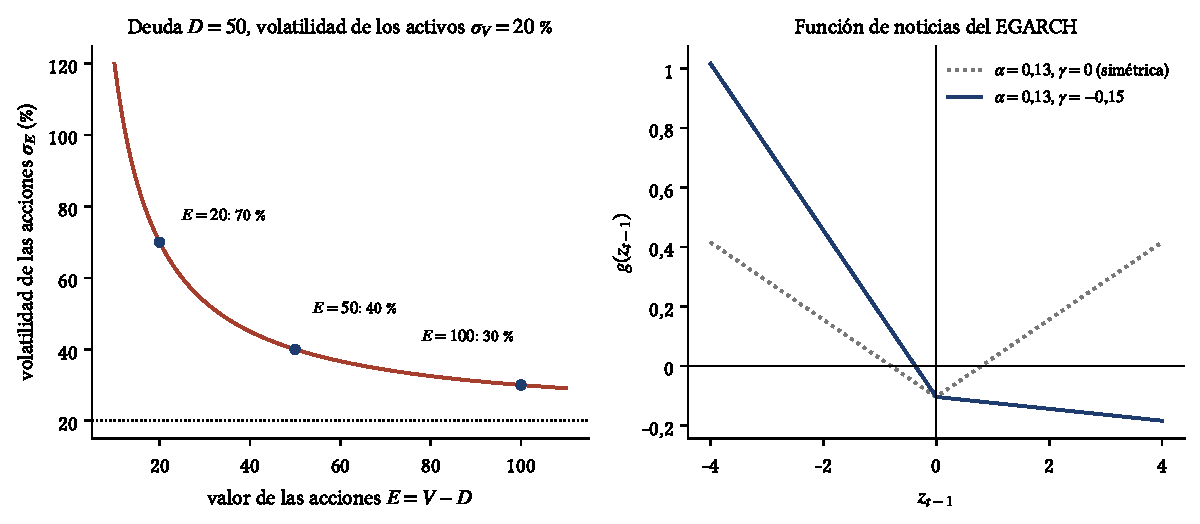
\includegraphics[width=\linewidth]{graficos/cap09_fig_apalancamiento.pdf}
\caption{Izquierda: volatilidad de las acciones según la Proposición~\ref{prop:black} cuando cae el valor de la
empresa; la línea punteada es la volatilidad de los activos. Derecha: función de noticias $g(z)$ del EGARCH,
simétrica con $\gamma=0$ y con pendiente mucho mayor para los choques negativos con $\gamma<0$.}
\label{fig:apalanc}
\end{figure}

% ---------------------------------------------------------------------
\section{Modelos GARCH asimétricos}
% ---------------------------------------------------------------------

\subsection{GJR-GARCH}

\begin{definicion}[GJR-GARCH(1,1); Glosten, Jagannathan y Runkle, 1993]
Sea $I_{t-1}=1$ si $\varepsilon_{t-1}<0$ e $I_{t-1}=0$ en otro caso.
\[
  \sigma_t^2=\omega+\bigl(\alpha+\gamma\,I_{t-1}\bigr)\varepsilon_{t-1}^2+\beta\,\sigma_{t-1}^2,
  \qquad \omega>0,\ \alpha\ge0,\ \alpha+\gamma\ge0,\ \beta\ge0 .
\]
\end{definicion}

Una buena noticia ($\varepsilon_{t-1}>0$) entra con coeficiente $\alpha$; una mala, con $\alpha+\gamma$. Si
$\gamma>0$, hay efecto apalancamiento; $\gamma=0$ devuelve el GARCH(1,1).

\begin{proposicion}[Varianza incondicional del GJR-GARCH]\label{prop:gjr}
Si la distribución de $z_t$ es simétrica alrededor de cero y $\alpha+\gamma/2+\beta<1$,
\[
  \bar\sigma^2=\frac{\omega}{1-\alpha-\gamma/2-\beta}.
\]
\end{proposicion}

\begin{proof}
Primero, por la simetría de $z$, la mitad del segundo momento proviene de los valores negativos:
\begin{align*}
  1 &= \E[z^2]\\
    &= \E\bigl[z^2\,\mathbf 1(z<0)\bigr]+\E\bigl[z^2\,\mathbf 1(z>0)\bigr]\\
    &= 2\,\E\bigl[z^2\,\mathbf 1(z<0)\bigr],\\[4pt]
  \E\bigl[z^2\,\mathbf 1(z<0)\bigr] &= \tfrac12 .
\end{align*}
Como $\varepsilon_{t-1}=\sigma_{t-1}z_{t-1}$ e $I_{t-1}=\mathbf 1(z_{t-1}<0)$, con $\sigma_{t-1}$ independiente de
$z_{t-1}$:
\begin{align*}
  \E\bigl[I_{t-1}\varepsilon_{t-1}^2\bigr] &= \E[\sigma_{t-1}^2]\,\E\bigl[z^2\,\mathbf 1(z<0)\bigr]\\
                                          &= \tfrac12\,\bar\sigma^2 .
\end{align*}
Tomamos esperanzas en la ecuación del modelo:
\begin{align*}
  \bar\sigma^2 &= \omega+\alpha\bar\sigma^2+\gamma\cdot\tfrac12\bar\sigma^2+\beta\bar\sigma^2,\\
  \bar\sigma^2\bigl(1-\alpha-\tfrac\gamma2-\beta\bigr) &= \omega,\\
  \bar\sigma^2 &= \frac{\omega}{1-\alpha-\gamma/2-\beta}. && \qedhere
\end{align*}
\end{proof}

La persistencia del GJR es $\alpha+\gamma/2+\beta$: el término asimétrico cuenta la mitad porque solo actúa la
mitad de las veces. Su pronóstico tiene la misma forma que el de la Proposición~\ref{prop:garchpron}, con esa
persistencia en lugar de $\alpha+\beta$.

\subsection{EGARCH}

\begin{definicion}[EGARCH(1,1); Nelson, 1991]
Con $z_{t-1}=\varepsilon_{t-1}/\sigma_{t-1}$,
\[
  \ln\sigma_t^2=\omega+g(z_{t-1})+\beta\ln\sigma_{t-1}^2,\qquad
  g(z)=\alpha\bigl(|z|-\E|z|\bigr)+\gamma\,z .
\]
\end{definicion}

El modelo tiene tres ventajas. Como se modela el logaritmo, $\sigma_t^2=e^{\ln\sigma_t^2}$ es siempre positiva
y no hacen falta restricciones de signo. La función $g$ es lineal por tramos (Figura~\ref{fig:apalanc},
derecha): su pendiente es $\alpha+\gamma$ para $z>0$ y $\gamma-\alpha$ para $z<0$, de modo que con $\gamma<0$ los
choques negativos pesan más. Y los choques entran estandarizados, en unidades de desviación estándar.

\begin{proposicion}[Media de $|z|$ y estacionariedad del EGARCH]\label{prop:egarch}
En el EGARCH(1,1):
\begin{enumerate}[label=(\roman*)]
  \item Si $z\sim N(0,1)$, $\E|z|=\sqrt{2/\pi}\approx0{,}7979$, de modo que $\E[g(z)]=0$.
  \item Si $|\beta|<1$, el logaritmo $\ln\sigma_t^2$ sigue un AR(1) estacionario, cuya media es
        $\omega/(1-\beta)$.
\end{enumerate}
\end{proposicion}

\begin{proof}
(i) Por simetría, $\E|z|$ es el doble de la integral sobre los positivos. Como
$\frac{d}{dz}\bigl(-e^{-z^2/2}\bigr)=z\,e^{-z^2/2}$,
\begin{align*}
  \E|z| &= 2\int_0^\infty z\,\frac{1}{\sqrt{2\pi}}e^{-z^2/2}\,dz\\
        &= \frac{2}{\sqrt{2\pi}}\Bigl[-e^{-z^2/2}\Bigr]_0^\infty\\
        &= \frac{2}{\sqrt{2\pi}}\,(0+1)\\
        &= \sqrt{\frac{2}{\pi}} .
\end{align*}
Entonces
\begin{align*}
  \E[g(z)] &= \alpha\bigl(\E|z|-\E|z|\bigr)+\gamma\,\E[z]\\
           &= 0+0\\
           &= 0 .
\end{align*}
(ii) Con $y_t=\ln\sigma_t^2$ y $u_t=g(z_{t-1})$, que son i.i.d.\ con media cero, la ecuación es
$y_t=\omega+\beta y_{t-1}+u_t$, un AR(1). Si $|\beta|<1$ es estacionario y, tomando esperanzas,
\begin{align*}
  \E[y] &= \omega+\beta\,\E[y],\\
  \E[y] &= \frac{\omega}{1-\beta}. && \qedhere
\end{align*}
\end{proof}

En el EGARCH la persistencia es $\beta$ y se refiere al logaritmo de la varianza. Si las innovaciones son $t$
de Student, $\E|z|$ ya no es $\sqrt{2/\pi}$; la biblioteca \texttt{arch} y nuestras funciones conservan
$\sqrt{2/\pi}$ como constante de centrado, lo que solo cambia el valor de $\omega$.

\subsection{Curvas de impacto de noticias}

Engle y Ng (1993) propusieron comparar modelos mediante su \emph{curva de impacto de noticias}: la varianza de
mañana, $\sigma_t^2$, como función del choque de hoy, $\varepsilon_{t-1}$, manteniendo fija la varianza de hoy
$\sigma_{t-1}^2$ en un valor típico. La Figura~\ref{fig:nicteo} compara las tres formas con parámetros que dan la
misma persistencia: el GARCH es una parábola simétrica; el GJR, una parábola con dos ramas de distinta
curvatura que se unen en cero; el EGARCH, una curva exponencial asimétrica que crece más despacio para los
choques extremos.

\begin{figure}[ht]
\centering
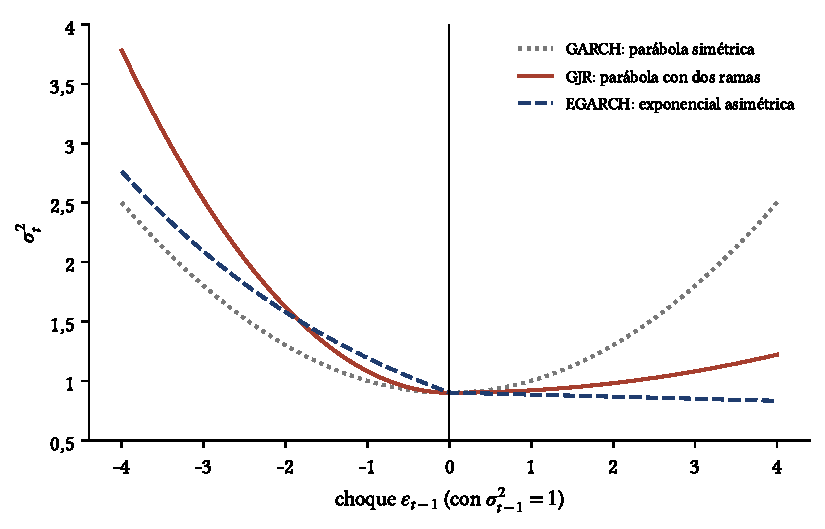
\includegraphics[width=0.72\linewidth]{graficos/cap09_fig_nic_teoria.pdf}
\caption{Curvas de impacto de noticias teóricas con $\sigma_{t-1}^2=1$. GARCH: $\omega=0{,}02$, $\alpha=0{,}10$,
$\beta=0{,}88$. GJR: $\omega=0{,}02$, $\alpha=0{,}02$, $\gamma=0{,}16$, $\beta=0{,}88$. EGARCH: $\omega=0$,
$\alpha=0{,}13$, $\gamma=-0{,}15$, $\beta=0{,}98$.}
\label{fig:nicteo}
\end{figure}

% ---------------------------------------------------------------------
\section{Pruebas de sesgo de signo}
% ---------------------------------------------------------------------

¿Cómo saber si un modelo simétrico deja sin capturar alguna asimetría? Engle y Ng (1993) proponen estimar un
modelo simétrico, calcular los residuos estandarizados $\hat z_t$ y estimar por MCO
\[
  \hat z_t^2=b_0+b_1S^-_{t-1}+b_2S^-_{t-1}\hat z_{t-1}+b_3S^+_{t-1}\hat z_{t-1}+u_t,
\]
donde $S^-_{t-1}=1$ si $\hat z_{t-1}<0$ y $S^+_{t-1}=1-S^-_{t-1}$. Si el modelo es correcto, $\hat z_t^2$ no
debería depender del pasado y los tres coeficientes deberían ser cero:
\begin{itemize}[leftmargin=*]
  \item $b_1$ (\emph{sesgo de signo}): ¿los choques negativos, sin importar su tamaño, elevan la volatilidad más
        de lo que predice el modelo?
  \item $b_2$ (\emph{sesgo de tamaño negativo}): ¿los choques negativos grandes la elevan más que los pequeños?
  \item $b_3$ (\emph{sesgo de tamaño positivo}): lo mismo para los choques positivos.
\end{itemize}
La prueba conjunta usa $LM=(T-1)R^2\xrightarrow{d}\chi^2_3$, con $T-1$ observaciones en la regresión.

% ---------------------------------------------------------------------
\section{GARCH en media: riesgo y rendimiento}
% ---------------------------------------------------------------------

La teoría de carteras dice que los inversionistas aversos al riesgo exigen un premio por soportarlo. Merton
(1980) muestra que, en un modelo de equilibrio intertemporal sencillo, el exceso de rendimiento esperado del
mercado es proporcional a su varianza condicional,
\[
  \E_{t-1}\bigl[r^e_t\bigr]=A\,\sigma_t^2,
\]
donde $A$ es el coeficiente de aversión relativa al riesgo del inversionista representativo. Engle, Lilien y
Robins (1987) propusieron llevar esa idea a la ecuación de la media de un GARCH.

\begin{definicion}[GARCH en media]
\[
  r^e_t=\mu+\lambda\,\sigma_t^2+\varepsilon_t,\qquad \varepsilon_t=\sigma_tz_t,\qquad
  \sigma_t^2=\omega+\alpha\varepsilon_{t-1}^2+\beta\sigma_{t-1}^2 .
\]
\end{definicion}

El modelo de Merton predice $\mu=0$ y $\lambda=A>0$. Hay que cuidar las unidades: si los rendimientos se miden
en porcentaje, $\tilde r^e=100\,r^e$ y $\tilde\sigma^2=10^4\sigma^2$, y la ecuación $\tilde r^e=\lambda\,\tilde\sigma^2$
equivale a
\begin{align*}
  100\,r^e &= \lambda\cdot10^4\,\sigma^2,\\
  r^e      &= 100\,\lambda\,\sigma^2,
\end{align*}
de modo que la aversión al riesgo implícita es $A=100\,\lambda$. La estimación es delicada: la media de los
rendimientos se estima con mucha imprecisión (Capítulo~\ref{cap:rendimientos}), y $\lambda$ aún más. Además, en
este modelo los errores en la ecuación de la varianza contaminan la de la media, porque ambas se estiman a la
vez. Las funciones del capítulo permiten estimar el GARCH-M, el GJR-M y el EGARCH-M con la misma recursión: la
innovación es $\varepsilon_t=r_t-\mu-\lambda\sigma_t^2$, y $\sigma_t^2$ depende de $\varepsilon_{t-1}$.

% ---------------------------------------------------------------------
\section{Ejercicios resueltos}
% ---------------------------------------------------------------------

\begin{ejresuelto}{¿Hay asimetría en el S\&P 500 y en el Brent?}\label{ej:asim}
\enunciado Para los rendimientos diarios del S\&P 500 (1999--2018) y del Brent (1987--2026): (a) calcule
$\operatorname{corr}(r_{t-j},r_t^2)$ y $\operatorname{corr}(r_{t-j}^2,r_t)$ para $j=1,\dots,10$; (b) estime un
GARCH(1,1) normal y aplique las pruebas de sesgo de signo de Engle y Ng a sus residuos estandarizados.

\solucion
\paso{Paso 1. Correlaciones cruzadas.} En el S\&P 500 las correlaciones entre el rendimiento pasado y la
volatilidad presente son negativas en los diez rezagos, entre $-0{,}113$ y $-0{,}036$, todas fuera de la
banda $\pm1{,}96/\sqrt{5\,030}=\pm0{,}028$: los días de caída anuncian días de más volatilidad durante dos
semanas. Las correlaciones en sentido contrario, $\operatorname{corr}(r_{t-j}^2,r_t)$, son pequeñas y de signo
cambiante (Figura~\ref{fig:asim}). El Brent también muestra una correlación negativa en $j=1$ ($-0{,}117$), pero
las siguientes son pequeñas; su $\operatorname{corr}(r_{t-1}^2,r_t)=0{,}123$ es positiva y refleja sobre todo el
rebote del 22 de abril de 2020 después de la caída del día anterior.

\paso{Paso 2. Pruebas de Engle y Ng.}
\begin{center}\small
\begin{tabular}{@{}lrrrr@{}}
\toprule
 & \multicolumn{2}{c}{S\&P 500} & \multicolumn{2}{c}{Brent} \\
\cmidrule(lr){2-3}\cmidrule(lr){4-5}
Coeficiente & Estimación & $t$ & Estimación & $t$ \\
\midrule
$b_0$ constante             & 0,9942 & 16,18 & 0,9809 & 20,79 \\
$b_1$ sesgo de signo        & 0,1733 & 2,06 & 0,0967 & 1,47 \\
$b_2$ tamaño negativo       & 0,0353 & 0,66 & $-0{,}0005$ & $-0{,}01$ \\
$b_3$ tamaño positivo       & $-0{,}1891$ & $-2{,}82$ & $-0{,}0816$ & $-1{,}67$ \\
\midrule
$LM=(T-1)R^2$               & \multicolumn{2}{r}{34,09 ($p=1{,}9\times10^{-7}$)} & \multicolumn{2}{r}{15,36 ($p=0{,}0015$)} \\
\bottomrule
\end{tabular}
\end{center}
Con 3 grados de libertad, el valor crítico al 5\,\% es $7{,}81$: las dos series rechazan que el GARCH simétrico
sea suficiente. En el S\&P 500 el mensaje es claro: después de un choque negativo, $\hat z_t^2$ es en promedio
$0{,}17$ mayor de lo que el GARCH predice ($b_1$), y después de un choque positivo grande es menor ($b_3<0$). El
GARCH simétrico subestima la volatilidad tras las malas noticias y la sobrestima tras las buenas. En el Brent los
coeficientes tienen los mismos signos pero son menores e individualmente no significativos.

\codigoweb{cap09_ej01}
\salidaR{cap09_ej01_R.txt}
\lectura{cap09_ej01}

\RvsPy Las funciones de este capítulo generalizan las del Capítulo~\ref{cap:garch}: una sola recursión cubre el
GARCH, el GJR y el EGARCH, con o sin término en media, y la verosimilitud normal o $t$. Después del
optimizador (\texttt{nlminb} en R, \texttt{L-BFGS-B} en Python) se hacen pasos de Newton con reducción del paso
para afinar el máximo en los dos lenguajes por igual. Ambas funciones devuelven un valor muy grande si unos
parámetros de prueba hacen explotar la recursión, para que el optimizador los descarte. Las diferencias de
espacios en las salidas se deben a que \texttt{sprintf} de R cuenta bytes y la ``ñ'' ocupa dos.

\begin{figure}[ht]
\centering
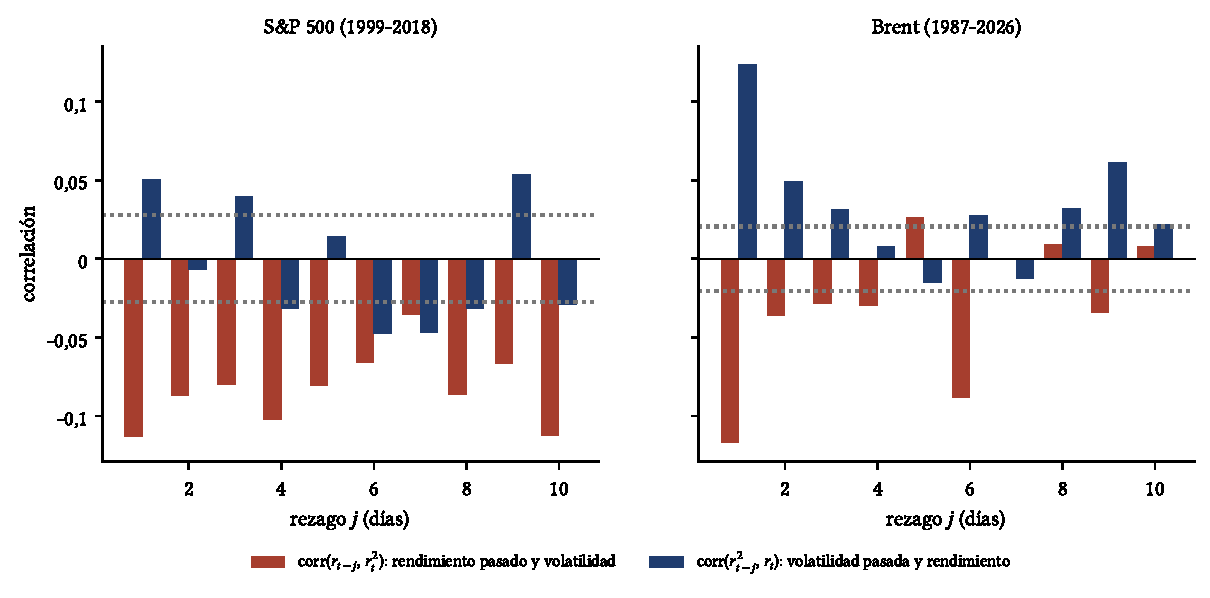
\includegraphics[width=\linewidth]{graficos/cap09_ej01_asimetria.pdf}
\caption{Correlaciones cruzadas entre rendimientos y rendimientos al cuadrado. En el S\&P 500 los rendimientos
pasados se correlacionan negativamente con la volatilidad presente durante al menos diez días.}
\label{fig:asim}
\end{figure}

\begin{conclusion}
El S\&P 500 tiene una asimetría marcada que el GARCH simétrico no captura. En el Brent la asimetría existe, pero
es mucho más débil.
\end{conclusion}
\end{ejresuelto}

\begin{ejresuelto}{GJR-GARCH para el S\&P 500 y comparación con el VIX}\label{ej:gjr}
\enunciado Estime un GJR-GARCH(1,1) con innovaciones $t$ para el S\&P 500 diario. Contraste $\gamma=0$ con una
prueba de razón de verosimilitudes frente al GARCH-$t$. Calcule la persistencia, la vida media y la volatilidad
incondicional. Compare la volatilidad anualizada estimada con el VIX.

\solucion
\paso{Paso 1. Estimación.}
\begin{center}\small
\begin{tabular}{@{}lrrr@{}}
\toprule
 & Coeficiente & ee robusto & $t$ \\
\midrule
$\mu$    & 0,0367 & 0,0104 & 3,52 \\
$\omega$ & 0,0132 & 0,0029 & 4,47 \\
$\alpha$ & 0,0000 & 0,0097 & 0,00 \\
$\gamma$ & 0,1815 & 0,0224 & 8,10 \\
$\beta$  & 0,8987 & 0,0132 & 68,06 \\
$\nu$    & 7,5042 & 0,8352 & 8,99 \\
\bottomrule
\end{tabular}
\end{center}
El resultado es extremo: $\hat\alpha$ llega a su cota de cero. Las buenas noticias no elevan en absoluto la
volatilidad del S\&P 500; solo las malas lo hacen, con coeficiente $\hat\alpha+\hat\gamma=0{,}1815$. (Cuando un
parámetro cae en la frontera, su error estándar y su $t$ no tienen la interpretación habitual.)

\paso{Paso 2. Razón de verosimilitudes.} El GARCH-$t$ simétrico tiene $\hat\ell=-6\,834{,}48$ y el GJR-$t$,
$\hat\ell=-6\,748{,}27$:
\begin{align*}
  LR &= 2\bigl(\hat\ell_{\text{GJR}}-\hat\ell_{\text{GARCH}}\bigr)\\
     &= 2\bigl(-6\,748{,}27+6\,834{,}48\bigr)\\
     &= 2\times86{,}21\\
     &= 172{,}42,
\end{align*}
frente a un valor crítico $\chi^2_1$ al 5\,\% de $3{,}84$ ($p\approx2\times10^{-39}$).

\paso{Paso 3. Persistencia y nivel de largo plazo.} Por la Proposición~\ref{prop:gjr}:
\begin{align*}
  \hat\phi &= \hat\alpha+\frac{\hat\gamma}2+\hat\beta\\
           &= 0+0{,}0907+0{,}8987\\
           &= 0{,}98944,\\[4pt]
  h_{1/2}  &= \frac{\ln0{,}5}{\ln0{,}98944}=65{,}3\ \text{días},\\[4pt]
  \hat{\bar\sigma}^2 &= \frac{0{,}0132}{1-0{,}98944}=1{,}2456 .
\end{align*}
La volatilidad anual de largo plazo es $\sqrt{252\times1{,}2456}=17{,}7$\,\%, algo menor que la muestral, de
19,1\,\%. La persistencia del S\&P 500 es claramente menor que la del Brent: sus choques se disipan en semanas,
no en trimestres.

\paso{Paso 4. Comparación con el VIX.} En los 5\,029 días comunes, la correlación entre la volatilidad
anualizada del GJR y el VIX es $0{,}900$. Pero el VIX es en promedio 3,04 puntos mayor (19,94 frente a 16,89).
La diferencia es la \emph{prima por riesgo de varianza}: los compradores de opciones pagan por protegerse de
aumentos de volatilidad, y la volatilidad implícita en los precios de las opciones supera en promedio a la que
luego se realiza (Figura~\ref{fig:gjrvix}).

\codigoweb{cap09_ej02}
\salidaR{cap09_ej02_R.txt}
\lectura{cap09_ej02}

\RvsPy Las dos implementaciones coinciden con \texttt{arch} en los coeficientes; $\hat\nu$ difiere en la cuarta
cifra decimal entre R ($7{,}5042$) y Python ($7{,}5041$) porque la verosimilitud es muy plana en esa dirección y
porque $\hat\alpha$ en la frontera impide el paso de Newton completo. Para cruzar las fechas con el VIX, R usa
\texttt{match} y Python \texttt{merge}.

\begin{figure}[ht]
\centering
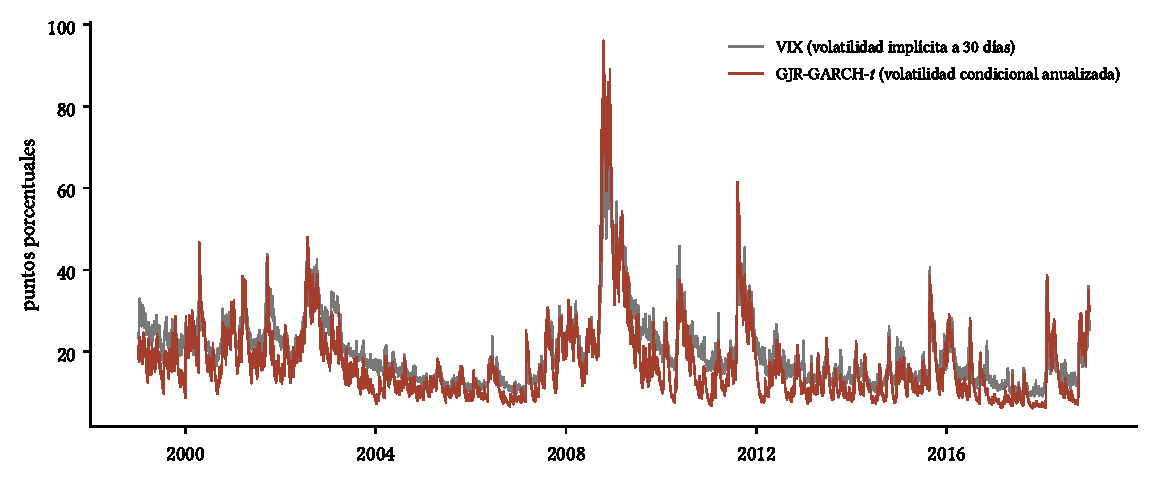
\includegraphics[width=0.92\linewidth]{graficos/cap09_ej02_gjr_vix.pdf}
\caption{Volatilidad condicional anualizada del S\&P 500 según el GJR-GARCH-$t$ y el VIX (1999--2018). Se mueven
juntas, pero el VIX suele estar por encima: es la prima por riesgo de varianza.}
\label{fig:gjrvix}
\end{figure}

\begin{conclusion}
En el S\&P 500 la volatilidad responde casi solo a las malas noticias. El GJR-GARCH mejora la verosimilitud en
86 puntos con un solo parámetro adicional y produce una volatilidad muy parecida a la que el mercado de opciones
incorpora en el VIX.
\end{conclusion}
\end{ejresuelto}

\begin{ejresuelto}{EGARCH y curvas de impacto de noticias del S\&P 500}\label{ej:egarch}
\enunciado Estime un EGARCH(1,1)-$t$ para el S\&P 500. Compare GARCH-$t$, GJR-$t$ y EGARCH-$t$ con AIC y BIC.
Dibuje sus curvas de impacto de noticias con $\sigma_{t-1}^2$ igual a la varianza muestral y calcule, para cada
modelo, el cociente entre la varianza que sigue a un choque de $-2$ y de $+2$ desviaciones estándar.

\solucion
\paso{Paso 1. Estimación.} $\hat\mu=0{,}0367$, $\hat\omega=-0{,}0021$, $\hat\alpha=0{,}1285$ ($t=8{,}96$),
$\hat\gamma=-0{,}1541$ ($t=-11{,}49$), $\hat\beta=0{,}9824$ y $\hat\nu=7{,}29$. Las pendientes de $g(z)$ son
\begin{align*}
  z>0:&\quad \hat\alpha+\hat\gamma=0{,}1285-0{,}1541=-0{,}0256,\\
  z<0:&\quad \hat\gamma-\hat\alpha=-0{,}1541-0{,}1285=-0{,}2826 .
\end{align*}
Para $z<0$, una pendiente negativa significa que la varianza \emph{sube} cuando $z$ se hace más negativo: un
choque de $-1$ eleva $\ln\sigma_t^2$ en $0{,}28$. Para $z>0$, la pendiente es casi nula y ligeramente negativa:
las buenas noticias \emph{reducen} un poco la volatilidad. La vida media de una perturbación en
$\ln\sigma^2$ es $\ln0{,}5/\ln0{,}9824=39{,}1$ días.

\paso{Paso 2. Comparación de modelos.}
\begin{center}\small
\begin{tabular}{@{}lrrrr@{}}
\toprule
Modelo & $k$ & $\hat\ell$ & AIC & BIC \\
\midrule
GARCH-$t$  & 5 & $-6\,834{,}48$ & 13\,678,96 & 13\,711,57 \\
GJR-$t$    & 6 & $-6\,748{,}27$ & 13\,508,54 & 13\,547,68 \\
EGARCH-$t$ & 6 & $-6\,732{,}24$ & 13\,476,49 & 13\,515,63 \\
\bottomrule
\end{tabular}
\end{center}
Los dos criterios eligen el EGARCH, con el mismo número de parámetros que el GJR y 16 puntos más de
log-verosimilitud. Los dos modelos asimétricos superan con holgura al simétrico.

\paso{Paso 3. Curvas de impacto.} Con $\sigma_{t-1}^2=1{,}4492$, un choque de dos desviaciones estándar es
$2\sqrt{1{,}4492}=2{,}408$\,\%. La varianza de mañana resulta:
\begin{center}\small
\begin{tabular}{@{}lrrr@{}}
\toprule
Modelo & $\sigma_t^2$ tras $-2{,}408$\,\% & $\sigma_t^2$ tras $+2{,}408$\,\% & Cociente \\
\midrule
GARCH-$t$  & 1,8899 & 1,8899 & 1,00 \\
GJR-$t$    & 2,3676 & 1,3156 & 1,80 \\
EGARCH-$t$ & 2,2820 & 1,2321 & 1,85 \\
\bottomrule
\end{tabular}
\end{center}
En el GJR, por ejemplo,
\begin{align*}
  \sigma_t^2(-) &= 0{,}0132+0{,}1815\times2{,}408^2+0{,}8987\times1{,}4492 = 2{,}3676,\\
  \sigma_t^2(+) &= 0{,}0132+0\times2{,}408^2+0{,}8987\times1{,}4492 = 1{,}3156 .
\end{align*}
Una caída de dos desviaciones estándar lleva la varianza de mañana a casi el doble que una subida del mismo
tamaño. La Figura~\ref{fig:nicsp} muestra las curvas completas: el GARCH simétrico sobrestima la reacción a las
subidas y subestima la reacción a las caídas.

\codigoweb{cap09_ej03}
\salidaR{cap09_ej03_R.txt}
\lectura{cap09_ej03}

\RvsPy Las tres implementaciones (R, Python y \texttt{arch}) coinciden. La curva de impacto del EGARCH se
programa con la misma ecuación de la recursión, con $z_{t-1}=\varepsilon_{t-1}/\sigma_{t-1}$.

\begin{figure}[ht]
\centering
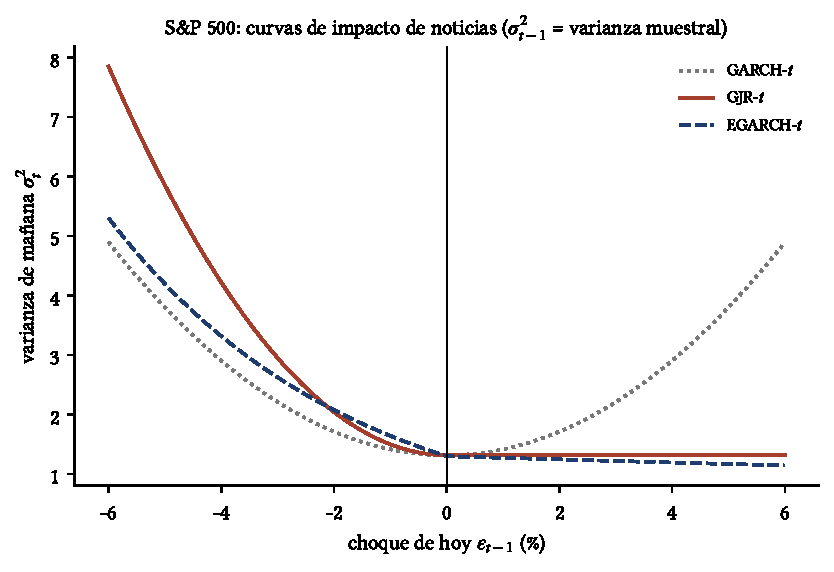
\includegraphics[width=0.74\linewidth]{graficos/cap09_ej03_nic_sp500.pdf}
\caption{Curvas de impacto de noticias estimadas para el S\&P 500. La rama derecha del GJR es plana porque
$\hat\alpha=0$; la del EGARCH desciende levemente porque $\hat\alpha+\hat\gamma<0$.}
\label{fig:nicsp}
\end{figure}

\begin{conclusion}
Los modelos asimétricos describen mucho mejor la volatilidad de las acciones. El EGARCH, que trabaja con
logaritmos y choques estandarizados, es el preferido por los criterios de información en esta muestra.
\end{conclusion}
\end{ejresuelto}

\begin{ejresuelto}{¿Tiene el petróleo efecto apalancamiento?}\label{ej:asimbrent}
\enunciado Estime GARCH-$t$, GJR-$t$ y EGARCH-$t$ para el Brent. Contraste $\gamma=0$ en el GJR. Calcule el
cociente de impactos de choques de $\pm2$ desviaciones estándar y compare con el S\&P 500. Verifique que el
resultado no depende de los episodios extremos de 2020--2026 reestimando el GJR hasta 2019.

\solucion
\paso{Paso 1. GJR-$t$.} $\hat\alpha=0{,}0676$, $\hat\gamma=0{,}0314$ ($t=3{,}09$), $\hat\beta=0{,}9115$ y
$\hat\nu=5{,}27$. La razón de verosimilitudes frente al GARCH-$t$ es
\begin{align*}
  LR &= 2\bigl(-19\,747{,}20+19\,752{,}61\bigr)\\
     &= 10{,}81\quad(p=0{,}0010).
\end{align*}
Hay asimetría en el Brent, del mismo signo que en las acciones, y significativa.

\paso{Paso 2. Magnitud.} En el GJR el coeficiente de $\varepsilon_{t-1}^2$ es $0{,}0990$ para las caídas y
$0{,}0676$ para las subidas:
\begin{align*}
  \frac{\hat\alpha+\hat\gamma}{\hat\alpha} &= \frac{0{,}0990}{0{,}0676}\\
                                         &= 1{,}46 .
\end{align*}
En el S\&P 500 ese cociente es infinito ($\hat\alpha=0$). Para un choque de dos desviaciones estándar ($5{,}408$\,\%),
el cociente de varianzas es $1{,}11$ en el GJR y $1{,}13$ en el EGARCH, frente a $1{,}80$ y $1{,}85$ en el
S\&P 500. La Figura~\ref{fig:nicbrent} compara las dos curvas en unidades comparables: la del Brent es casi
simétrica; la del S\&P 500 tiene una sola rama.

\paso{Paso 3. Comparación de modelos.}
\begin{center}\small
\begin{tabular}{@{}lrrrr@{}}
\toprule
Modelo & $k$ & $\hat\ell$ & AIC & BIC \\
\midrule
GARCH-$t$  & 5 & $-19\,752{,}61$ & 39\,515,21 & 39\,550,81 \\
GJR-$t$    & 6 & $-19\,747{,}20$ & 39\,506,40 & 39\,549,11 \\
EGARCH-$t$ & 6 & $-19\,722{,}71$ & 39\,457,42 & 39\,500,13 \\
\bottomrule
\end{tabular}
\end{center}
El EGARCH vuelve a ganar, pero aquí su ventaja no viene de la asimetría ($\hat\gamma=-0{,}0304$ es pequeña),
sino de su forma logarítmica, que responde con menos violencia a los choques enormes del Brent.

\paso{Paso 4. Robustez.} Con datos hasta 2019 ($T=7\,390$), $\hat\gamma=0{,}0301$ ($t=3{,}24$): la asimetría es
la misma sin la pandemia ni el año 2026.

\codigoweb{cap09_ej04}
\salidaR{cap09_ej04_R.txt}
\lectura{cap09_ej04}

\RvsPy En el EGARCH del Brent, R y Python se detienen en puntos que difieren en la cuarta decimal de $\hat\mu$
($0{,}0384$ frente a $0{,}0385$), con log-verosimilitudes que difieren en $0{,}00001$. La verosimilitud del EGARCH
no es derivable en todos los puntos (contiene $|z_{t-1}|$, y $z_{t-1}$ depende de $\mu$) y es casi plana en esa
dirección, así que el paso de Newton no puede afinar más; la diferencia no tiene ninguna consecuencia práctica.

\begin{figure}[ht]
\centering
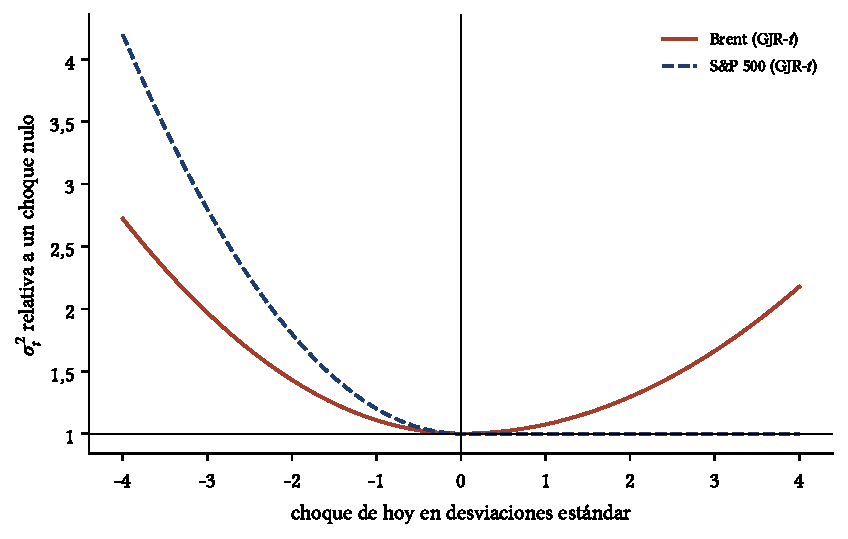
\includegraphics[width=0.74\linewidth]{graficos/cap09_ej04_nic_brent.pdf}
\caption{Curvas de impacto del GJR-$t$ en unidades de desviación estándar, relativas a la varianza tras un choque
nulo. El Brent responde de forma casi simétrica; el S\&P 500 solo a las caídas.}
\label{fig:nicbrent}
\end{figure}

\begin{conclusion}
El Brent tiene un efecto apalancamiento estadísticamente significativo, pero pequeño. Tiene sentido: en el
petróleo, las subidas bruscas del precio (por ejemplo, ante interrupciones de la oferta) también son noticias
que generan incertidumbre, mientras que la explicación por apalancamiento financiero no se aplica a una materia
prima.
\end{conclusion}
\end{ejresuelto}

\begin{ejresuelto}{GARCH en media: ¿pagan más las acciones cuando son más riesgosas?}\label{ej:garchm}
\enunciado Con el exceso de rendimiento mensual del mercado de EE.\,UU. (1926--2018, en porcentaje), estime un
GARCH-M con innovaciones normales y $t$, y un GJR-M con innovaciones $t$. Contraste $\lambda=0$, calcule la prima
implícita para la varianza promedio e interprete $\lambda$ como aversión al riesgo.

\solucion
\paso{Paso 1. Estimaciones.} Con $T=1\,109$ meses (media $0{,}66$\,\% mensual, varianza $28{,}38$):
\begin{center}\small
\begin{tabular}{@{}lrrrrr@{}}
\toprule
Modelo & $\hat\lambda$ & ee robusto & $t$ & Prima anual & $A=100\hat\lambda$ \\
\midrule
GARCH-M normal & 0,01167 & 0,00877 & 1,33 & 4,07\,\% & 1,17 \\
GARCH-M $t$    & 0,00872 & 0,00881 & 0,99 & 2,95\,\% & 0,87 \\
GJR-M $t$      & 0,00408 & 0,01115 & 0,37 & 1,34\,\% & 0,41 \\
\bottomrule
\end{tabular}
\end{center}
La prima es $\hat\lambda$ por la varianza condicional promedio, multiplicada por 12. Para el GARCH-M normal,
$0{,}3390\times12=4{,}07$\,\%.

\paso{Paso 2. Interpretación.} Los tres $\hat\lambda$ son positivos, como predice la teoría, y las aversiones
al riesgo implícitas (entre 0,4 y 1,2) son razonables. Pero ninguno es significativo, y la estimación cae a la
mitad o menos cuando se permite la asimetría. Es el resultado que encontraron Glosten, Jagannathan y Runkle
(1993): una vez que se modela que las caídas elevan la volatilidad, la relación positiva entre varianza y
rendimiento esperado se debilita o desaparece. En el GARCH-M simétrico, parte de $\hat\lambda$ captura
sencillamente que los meses de varianza alta suelen seguir a rebotes.

\paso{Paso 3. La prima en el tiempo.} Según el GARCH-M $t$, el exceso esperado anualizado
$12(\hat\mu+\hat\lambda\hat\sigma_t^2)$ llegó a casi 50\,\% en septiembre de 1932, cuando la volatilidad anualizada
alcanzó 68\,\%
(Figura~\ref{fig:garchm}). Ese tipo de predicciones extremas es otra razón para desconfiar de una relación lineal
entre la varianza y la media.

\codigoweb{cap09_ej05}
\salidaR{cap09_ej05_R.txt}
\lectura{cap09_ej05}

\RvsPy El GARCH-M se estima con las mismas funciones, indicando \texttt{media = "m"}. Acotamos $\lambda$ entre
$-0{,}5$ y $0{,}5$: sin cota, durante la búsqueda el optimizador de Python probaba valores que hacían explotar la
recursión. \texttt{arch} no incluye el GARCH en media, así que la verificación es entre R y Python, que coinciden
en todas las cifras.

\begin{figure}[ht]
\centering
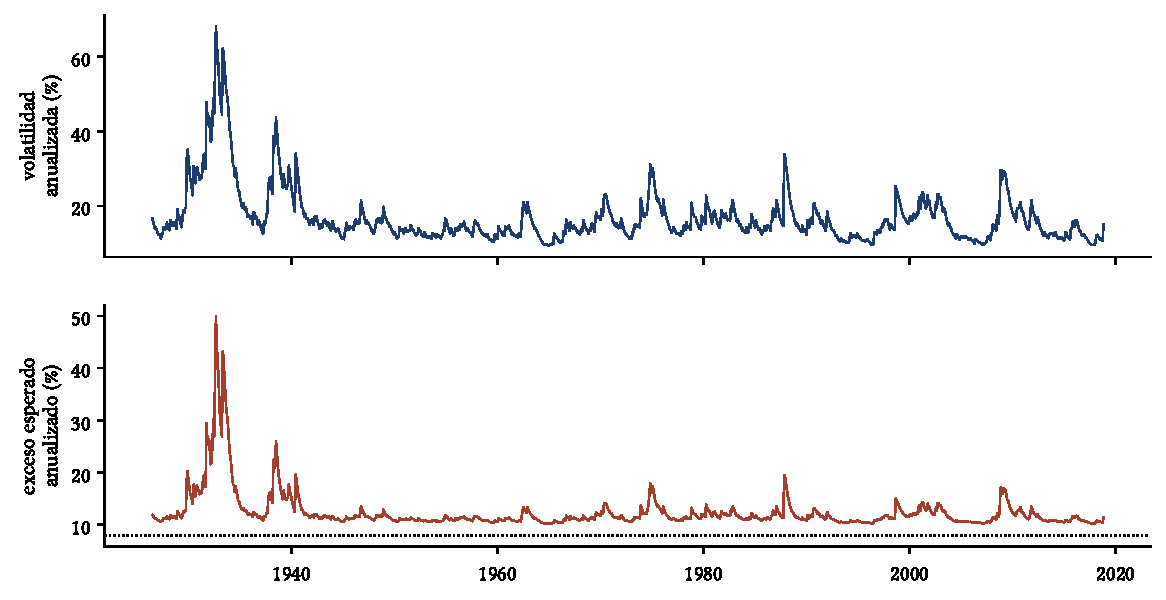
\includegraphics[width=0.92\linewidth]{graficos/cap09_ej05_garch_m.pdf}
\caption{GARCH-M $t$ para el exceso de rendimiento del mercado (1926--2018). Arriba: volatilidad condicional
anualizada. Abajo: exceso de rendimiento esperado anualizado; la línea punteada es el promedio muestral.}
\label{fig:garchm}
\end{figure}

\begin{conclusion}
Los datos son compatibles con una relación positiva entre riesgo y rendimiento esperado, pero no permiten
establecerla con confianza. La relación riesgo-rendimiento en el tiempo sigue siendo una de las preguntas
abiertas de la econometría financiera.
\end{conclusion}
\end{ejresuelto}

% ---------------------------------------------------------------------
\section{Ejercicios propuestos}
% ---------------------------------------------------------------------

\begin{enumerate}[label=\textbf{\thechapter.\arabic*},leftmargin=*,itemsep=6pt]
  \item Para un GJR-GARCH con $\omega=0{,}02$, $\alpha=0{,}03$, $\gamma=0{,}10$ y $\beta=0{,}90$, calcule la
  persistencia, la varianza incondicional y la vida media. \textit{Respuesta: $0{,}98$; $1$; $34{,}3$ períodos.}

  \item En un EGARCH con $\alpha=0{,}13$ y $\gamma=-0{,}15$ e innovaciones normales, calcule $g(2)$ y $g(-2)$, y el
  cociente $e^{g(-2)}/e^{g(2)}$. \textit{Respuesta: $-0{,}1437$; $0{,}4563$; $1{,}822$.}

  \item Una empresa tiene activos de 150, deuda sin riesgo de 60 y volatilidad de activos de 15\,\%. Calcule la
  volatilidad de sus acciones antes y después de que los activos caigan a 100. \textit{Respuesta: 25\,\% y
  37,5\,\%.}

  \item Demuestre que, para la $t$ estandarizada con $\nu$ grados de libertad,
  \[
    \E|z|=\frac{2\sqrt{\nu-2}\;\Gamma\bigl(\frac{\nu+1}2\bigr)}{\sqrt\pi\,(\nu-1)\,\Gamma\bigl(\frac\nu2\bigr)} .
  \]
  Evalúela en $\nu=7{,}2855$ y compárela con $\sqrt{2/\pi}$. \textit{Respuesta: $0{,}7612$ frente a $0{,}7979$.}

  \item Demuestre que en el GJR-GARCH el pronóstico de la varianza es
  $\E_T[\sigma_{T+h}^2]=\bar\sigma^2+\phi^{h-1}(\sigma_{T+1}^2-\bar\sigma^2)$ con $\phi=\alpha+\gamma/2+\beta$.

  \item \emph{(Simulación.)} Simule 500 muestras de 2\,000 observaciones de un GJR-GARCH normal con los
  parámetros del ejercicio 9.1, estime un GARCH(1,1) simétrico y aplique la prueba conjunta de Engle y Ng. ¿Con
  qué frecuencia detecta la asimetría?

  \item \emph{(Con datos.)} El paquete \texttt{arch} incluye el índice Nasdaq diario de 1999 a 2018
  (\texttt{arch.data.nasdaq}). Estime el GJR-$t$ y el EGARCH-$t$ y compare la asimetría y la persistencia con las
  del S\&P 500.

  \item \emph{(Con datos de Yahoo Finance.)} Descargue el índice S\&P/BVL Perú General y las acciones de
  Southern Copper (SCCO) y Credicorp (BAP). ¿Muestran efecto apalancamiento? ¿Es mayor en el banco, más
  endeudado, que en la minera?
\end{enumerate}

% ---------------------------------------------------------------------
\section{Resumen de fórmulas}
% ---------------------------------------------------------------------

\begin{table}[H]
\centering\small
\begin{tabular}{@{}ll@{}}
\toprule
Concepto & Fórmula \\
\midrule
Apalancamiento & $\sigma_E=(1+D/E)\,\sigma_V$ \\
GJR-GARCH & $\sigma_t^2=\omega+(\alpha+\gamma I_{t-1})\varepsilon_{t-1}^2+\beta\sigma_{t-1}^2$ \\
Persistencia GJR & $\alpha+\gamma/2+\beta$;\quad $\bar\sigma^2=\omega/(1-\alpha-\gamma/2-\beta)$ \\
EGARCH & $\ln\sigma_t^2=\omega+\alpha(|z_{t-1}|-\sqrt{2/\pi})+\gamma z_{t-1}+\beta\ln\sigma_{t-1}^2$ \\
Pendientes de $g(z)$ & $\alpha+\gamma$ si $z>0$;\quad $\gamma-\alpha$ si $z<0$ \\
Engle-Ng & $\hat z_t^2=b_0+b_1S^-_{t-1}+b_2S^-_{t-1}\hat z_{t-1}+b_3S^+_{t-1}\hat z_{t-1}$;\quad $(T-1)R^2\sim\chi^2_3$ \\
GARCH-M & $r^e_t=\mu+\lambda\sigma_t^2+\varepsilon_t$;\quad $A=100\lambda$ (datos en \%) \\
\bottomrule
\end{tabular}
\caption{Fórmulas principales del Capítulo 9.}
\end{table}

\section*{Referencias}
\begin{itemize}[leftmargin=*]
  \item Black, F. (1976). Studies of stock price volatility changes. \emph{Proceedings of the 1976 Meetings of the
        American Statistical Association, Business and Economic Statistics Section}, 177--181.
  \item Campbell, J. Y. y Hentschel, L. (1992). No news is good news: An asymmetric model of changing volatility
        in stock returns. \emph{Journal of Financial Economics}, 31(3), 281--318.
  \item Engle, R. F., Lilien, D. M. y Robins, R. P. (1987). Estimating time varying risk premia in the term
        structure: The ARCH-M model. \emph{Econometrica}, 55(2), 391--407.
  \item Engle, R. F. y Ng, V. K. (1993). Measuring and testing the impact of news on volatility. \emph{Journal
        of Finance}, 48(5), 1749--1778.
  \item Figlewski, S. y Wang, X. (2000). Is the ``leverage effect'' a leverage effect? Documento de trabajo,
        New York University.
  \item Glosten, L. R., Jagannathan, R. y Runkle, D. E. (1993). On the relation between the expected value and
        the volatility of the nominal excess return on stocks. \emph{Journal of Finance}, 48(5), 1779--1801.
  \item Merton, R. C. (1980). On estimating the expected return on the market: An exploratory investigation.
        \emph{Journal of Financial Economics}, 8(4), 323--361.
  \item Nelson, D. B. (1991). Conditional heteroskedasticity in asset returns: A new approach.
        \emph{Econometrica}, 59(2), 347--370.
\end{itemize}
